%!TEX root = ../main.tex
\section{Overview}

Various articles and research paper has been studied to find the applicability of time series imputation and time-series forecasting in the wireless sensor network. Also, various techniques and algorithms available to deal with this problem are studied. It gave a clear picture of what the problem is and what are the measures that are taken and can be taken to solve the problem. It gave a clear insight into the problem statement and helped in shaping the organisation and direction of the thesis.

\section{Related Literature}


A lot of literature is present on missing time series data imputation. Only closely related is mentioned here.
T et al. \cite{21}, the author proposed a fusion long short-term memory-convolutional neural network model to predict the stock prices by combining features from different representations of data. This model outperforms here in the comparison of single models because here, LSTM+CNN both used to extract temporal features and image features.\cite{22} Verma et al. \cite{23}, the author worked on RNN based model and used Generic Sliding Window (GSW) to produce more training samples, i.e., more time-series data so that model can be trained easily. 
\\

The traditional methods, like ARIMA, SARIMA, etc., remove the non-stationary parts in the time series data and try to fit a parameterized stationary model. Further combination of ARIMA and Kalman Filter \cite{24, 25} is used by the space model and provides better results. Multivariate Imputation by Chained Equations \cite{26} initializes the values which are missing in time series data randomly, and then the elimination of each missing variable is done using the chain equations. Yi et al. \cite{27} proposed a multi-view learning-based method to impute the missing time series values in air quality data and attain a mean relative error of about 17\% for PM2.5. Wang et al. \cite{28} applied a collaborative filtering method to the recommendation system in order to fill the missing time series values. 
\\

Yuan et al. \cite{29}, the author applied the LSTM model on air pollution time series data and proves the LSTM model outperforms the statistical method like mean, moving average method, etc., and achieves better accuracy in predicting PM2.5 values of time series data. Che et al.\cite{30}, the author proposed a method called GRU-D, which is applied to health care data, on which it gives a remarkable performance. This method is based upon Gated Recurrent Unit for missing time series data imputation. Sutskever et al. \cite{31}, the author invented a seq2seq learning approach that used multi-layer LSTM to map the input sequence to a fixed dimensional vector and a deep LSTM to decode the target sentences from that vector. The authors used the WMT'14 dataset for English to French translation tasks. The Authors achieved a BLEU score of 34.8 on the entire test set. The authors also analyzed that reversing the source sentences can lead to an increase in the performance of LSTM by making optimization easier\cite{25}.
\\
 
Leke et al. \cite{32}, the author proposed an auto-encoder neural network to predict missing data in the forest fire data set from the UCI data repository by considering that a wireless sensor network usually monitors multiple parameters and used a common approach is to reconstruct the missing parameter based on other available parameters in the data sets. Cho et al. \cite{33}, the author invented the Recurrent Neural Network-based Encoder-Decoder novel model. This model consisted of two Recurrent Neural Networks. One of the RNN would be used to encode input sentences into a fixed-length vector, and the other would be used to decode the fixed-length vector. The proposed model is jointly trained to maximize the probability of target sequences conditioned on source sentences.
\\
 
In the above discussion, various literature in the field of missing time series data imputation has been discussed. With the study of these works, it is analyzed that machine learning or deep learning techniques can play an important role in the imputation of missing time series data\cite{34}. It is also analyzed and understood that this work would be done by implementing Encoder-Decoder architecture of sequence two sequence learning \cite{35, 36, 37}
\\

Data loss is a major problem in IoT devices because of various issues like fault in the devices. \cite{21}
\\
Various methods for predicting missing data are developed to overcome this problem. Machine learning is a branch of computer science gaining much popularity these days and deep learning is a subset of machine learning which can be used for finding un evident pattern in the data which can be used to find the relation in the time series data and then that relationship can be used for predicting the missing data collected \cite{21}. 
\\

Predicting the missing data in time series data collected by the sensor would help in data analysis forecast prediction, corrective measures can be taken.\cite{24}
Machine learning and deep learning algorithms are proved to be best in predicting the missing data in the time-series data. Fig 1 depicts the machine learning techniques used for data imputation.
\\

Artificial neural network (ANN) - 
ANN is a machine learning technique where the model is trained by feeding samples to the model with the label. Training samples are generated using various sliding window methods available. It gives a fair result. But the resource overhead is more as we go deep for increasing the accuracy of the model.\cite{25}

\begin{figure}[ht]
	\centering
	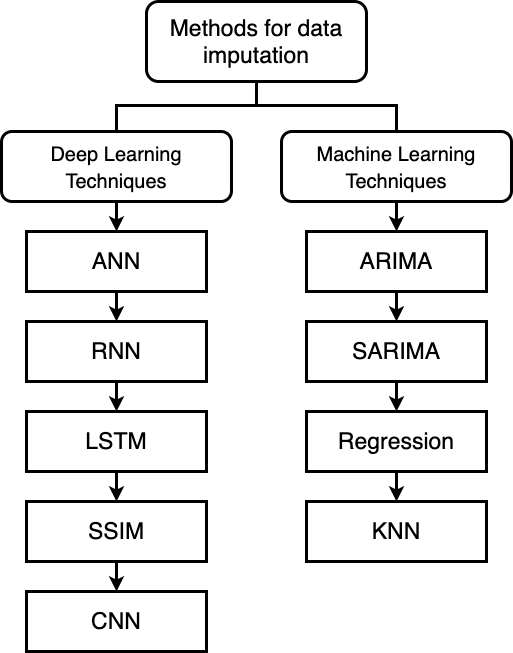
\includegraphics[width=0.5\textwidth]{images/algos.png}
	\caption{Available methods of imputation}
	\label{fig:algos}
\end{figure}

Recurrent Neural Network (RNN) - 
RNN is a machine learning technique in which temporal sequence is considered while making forecasting. Because of this reason it performs better than ANN. But still it is not capable to model upon large sequences of temporal data.\cite{26}
\\

Long Short Term Memory (LSTM) - 
The problem of remembering large sequence data and inferring upon it is overcome by LSTM network.\cite{27}
\\

Sequence to Sequence Imputation Model (SSIM) - 
In SSIM \cite{37} instead of predicting just the next data point in the sequence, it is capable of forecasting several data points next to the current end. Attention mechanism and (Variable length sliding window) VLSW are used for further improving the model accuracy/efficiency.\cite{28}
\\

Convolutional Neural Network (CNN) - 
The convolutional neural network is a technique in machine learning which is very famous in the image processing and video processing field. As it tries to learn the spatial arrangement of the pattern it proves to be useful in time series forecasting. But as it very resources heavy it may  not be suitable for IoT.\cite{29}
\\

\section{Summary}
Many machine learning and deep learning methods are available in the literature and can be used for making time series imputation and forecasting. Deep learning requires a large dataset to solve the problem effectively. WSN doesn't provide much data in the real-time scenario. There is also the limitation of applying deep learning of the scratch on end nodes due to low computing power and low memory available in the sensing nodes.